%-----------Chapter 6------------------------------------------
\chapter{eTourPlan And Its Evaluation on the Bhutan KB}

\hspace{0.3in}In this chapter, we describe the functionalities of our eTourPlan prototype considering different scenarios. We also demonstrate some experimental results of the key operations. Our illustrations of the operations are based on Bhutan KB. 

\hspace{0.3in}Bhutan is a popular tourist destination in Asia. Our Bhutan KB, described in Chapter 4, consists of profiles for 10 most popular provinces of 20 total in Bhutan, detailing a total of 23 attractions, 18 events, and 18 accommodations in these 10 provinces. The profile descriptions are based on real information, although we did not include each and every attractions and accommodations located in all the provinces. On top of the fact base on Bhutan, we have the rule subsystems described in Chapter 5, enriching the KB. We show how eTourPlan KB can be used to fulfill the need for retrieving precise tourist information of tourist entities in order to package a tour based on tourist's preferences. We also show how some of the rule subsystems can function as independent modules for various purposes. For example, the administrative partonomy of a country and the route planning module can be used as separate systems, not only for tourist services but also as a general knowledge portal for Bhutan.

\hspace{0.3in}The eTourPlan architecture is shown in Figure 6.1. The system is built on top of the rule engine, OO jDREW. This thesis is focused on knowledge acquisition and the application of rules on KB. However, future work of designing a convenient Graphical User Interface would help to emphasize the usefulness of the KB. We illustrate all the operations as tested using different queries on OO jDREW TD. First, the user posts a query to our eTourPlan system. The eTourPlan system then automatically applies the corresponding rules to the related tourism subdomain facts. After processing facts with rules, the result of the eTourPlan rule system may turn out be either a success or a failure. When the query is fullfiled by the system, eTourPlan shows the result bindings matched to the user's preferences. Otherwise, eTourPlan notifies the user that there is ``No Solution".  

\begin{figure}
\begin{center}
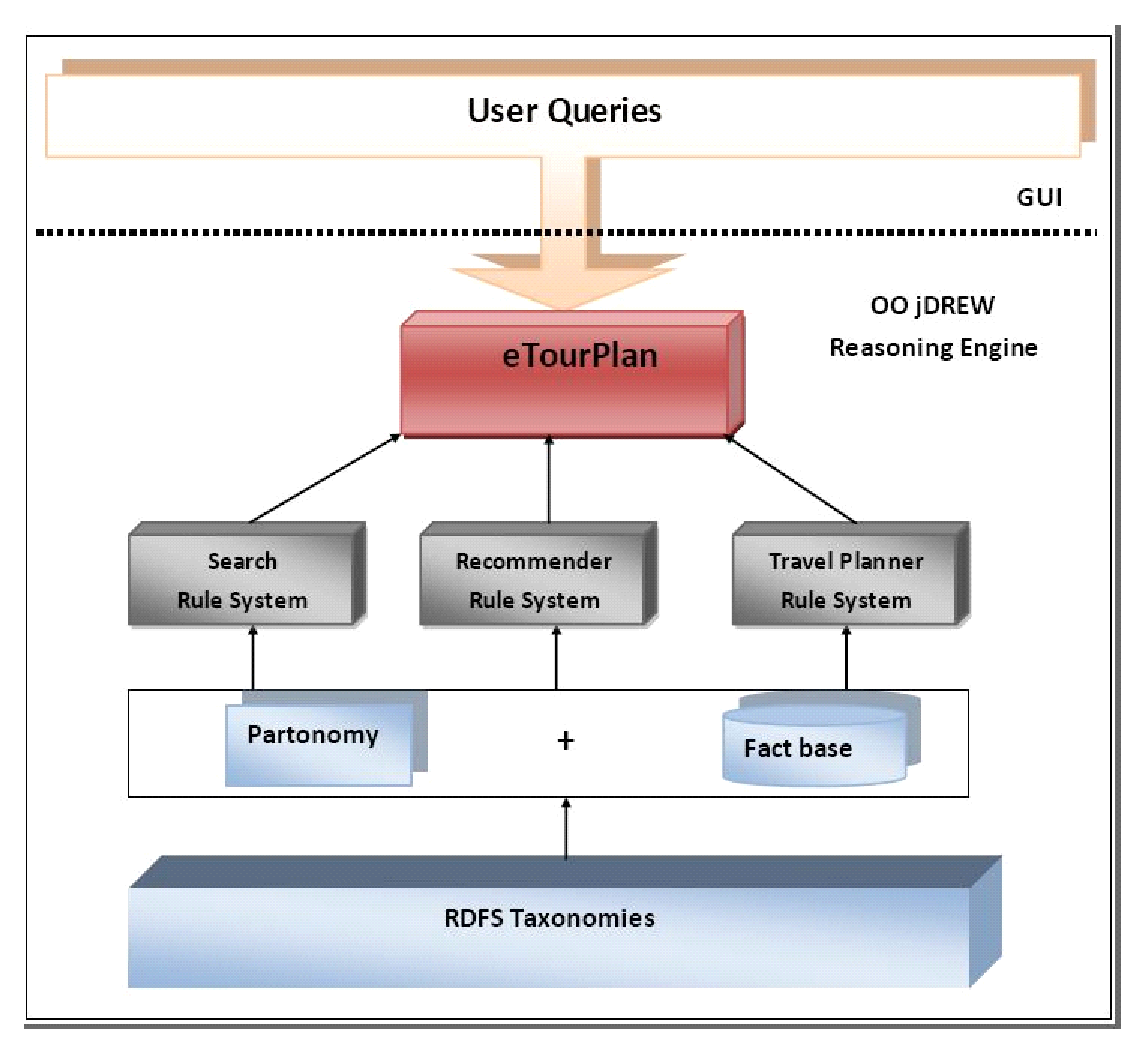
\includegraphics[width=12.5cm, height=8cm]{architecture}
\caption {eTourPlan Architecture}
\label{fig:Fig6.1}
\end{center}
\end{figure}

\section{Key Operations of the Prototype}
\hspace{0.3in} eTourplan prototype has three top-level categories of operations as shown in Figure 5.1. The operations are as follows:
\begin{itemize}
\item Search for information concerning tourist entities: provinces, attractions, events, and accommodation based on some preferences.
 \item Search route information between any two provinces. 
 \item  Provide travel route tailored to visiting user-preferred provinces
 \item Recommend touristic route of provinces
\item  Recommend a location-centric tour for a user-preferred provinces
\item  Generate an attraction-only travel plan 
\item  Generate events-only or event-centric with attraction recommendation travel plan
\end{itemize}

\section{OO jDREW TD User Interface}

\hspace{0.3in}The eTourPlan system is executed using the built-in OO jDREW TD interface (cf. the screen shot in Figure 6.2).  Brief directions for using the interface are given below:
\begin{enumerate}
\item Load the RDFS type definition file (by hand, from file) in the Type window (tab)
\item Load the KB in the Knowledge Base window (tab)
 \item Post your queries in the uppermost box in the Query Tab
 \item Click ``Issue Query" button to execute the eTourPlan system.
 \item After the eTourPlan computation is complete, result bindings will be shown on the righthand side of the interface. We can also trace how the results are bound in the result tree on the lefthand side of the interface.
 \item However, if eTourPlan system fails to find matching result bindings to the user's query, the lefthand side box for showing traces will remain ``No Solution". The box showing the result bindings will remain blank.
\end{enumerate}

\section{Experimental Results under Typical Operations}
\hspace{0.3in}In this section, we discuss how the eTourPlan system is tested under typical operations using varying types of different queries. Each of the subdomains are tested as separate module at first, and then together as a whole system, in order to verify the system operations. The following examples are used to demonstrate the typical operations in a bottom up fashion.

\subsection{Search operations}
\hspace{0.3in} Our KB consists of facts about the five main subdomains of tourism: events, attractions, accommodations, transportation, and geographic regions. This KB can be used for semantic information search on the tourism subdomains. For example, users can query for the details about any specific province, events, attractions, and accommodation from the KB. The search engine returns the result of the query based on user's preferences such as name or theme pertaining to a specific part of the country. One particularly good use of the search engine is for retrieving information concerning tourist entities pertaining to a specific subpart of the country. The search engine also provides route information between any two provinces. In this section, we describe some of typical search queries that can be issued against the different subdomains:\\

\subsubsection{Search for Provinces}
%%%%%%%%%%%%%%%%%%%%%%%%%%Table 6.1
\begin{table} [tbph]
\caption{Queries of different input/output modes for Province search}
\centering
\footnotesize
\begin{tabular}{|l|l|l|}
\hline
 Query&\textbf{User Input} &$~~~~~~~~~~~~~~~~~~~~$ \textbf{Query Formats} \\
 &$~~$\textbf{Values}   &$~~~~~~~~~~~~$(Input values are bold-faced)              \\
\hline
 1&$?$Name & getProvinceDetails(region-$>?$Region:Region;\\
  &        &$~~~~~~~~~~~~~~~~~~~~~~~~~~$name-$>$\textbf{Bumthang}:Province; \\
  &       &$~~~~~~~~~~~~~~~~~~~~~~~~~~?$ProvinceDetails)\\
          
 \hline
 2&$?$Region & getProvinceDetails(region-$>$\textbf{Central}:Region;\\
  &        &$~~~~~~~~~~~~~~~~~~~~~~~~~~$name-$>$?Name:Province; \\
  &        &$~~~~~~~~~~~~~~~~~~~~~~~~~~?$ProvinceDetails)\\
 \hline
 3&None & getProvinceDetails(region-$>?$Region:Region;\\
  &        &$~~~~~~~~~~~~~~~~~~~~~~~~~~$name-$>$?Name:Province; \\
  &        &$~~~~~~~~~~~~~~~~~~~~~~~~~~?$ProvinceDetails)\\         
\hline
\end{tabular} 
\end{table}


\begin{figure}
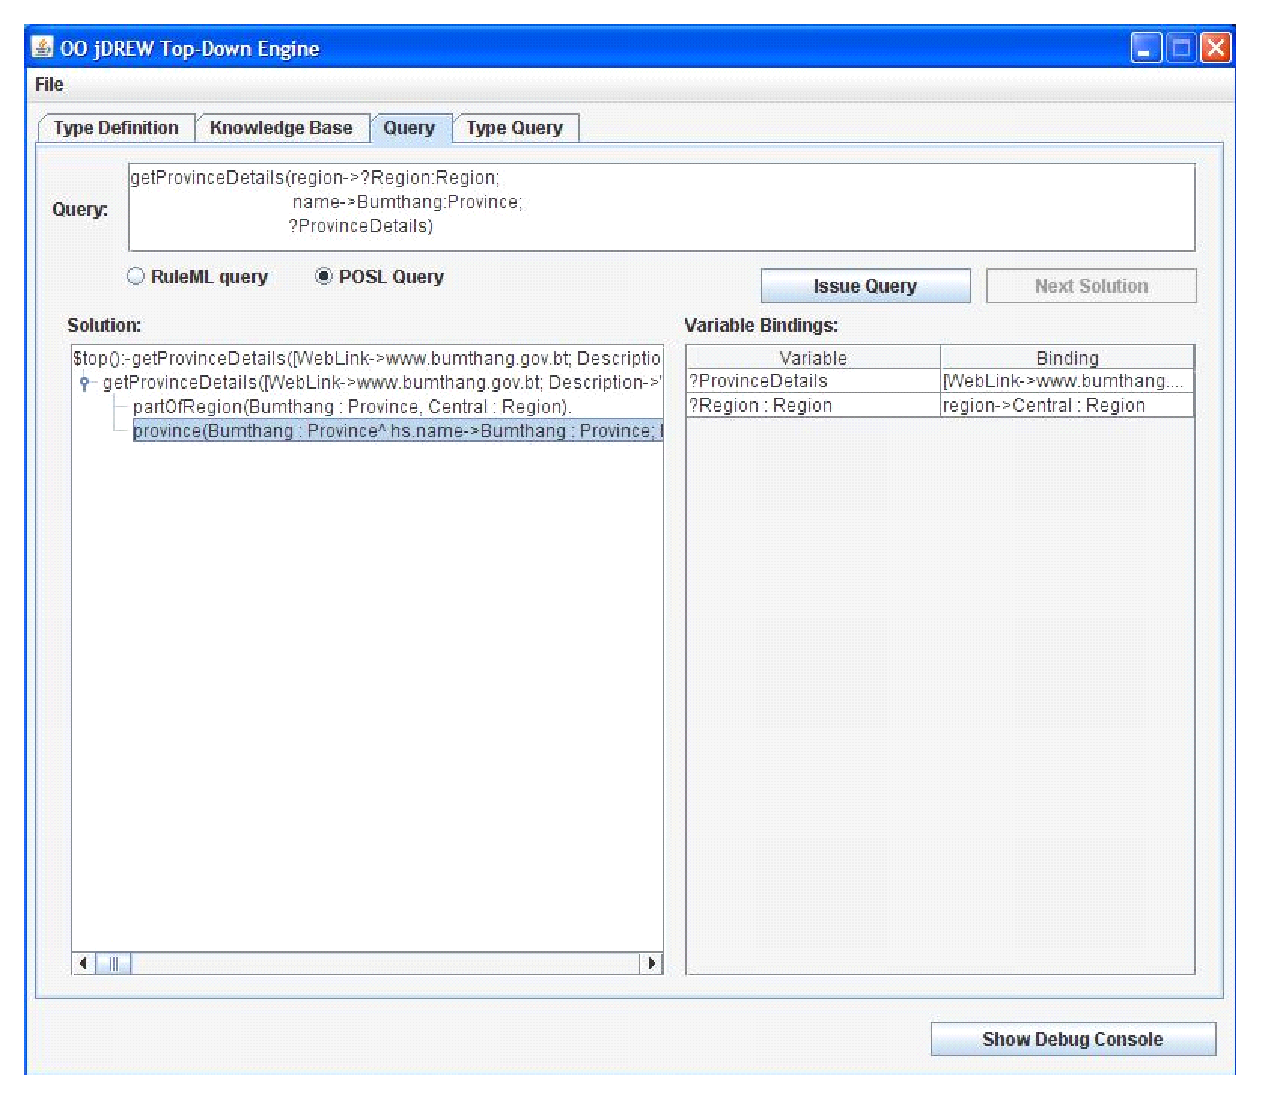
\includegraphics[width=6in]{screenshotProvince}
\caption {Screenshot for Query 1 result}
\label{fig:Fig6.2}
\end{figure}


\hspace{0.3in}The first query in Table 6.1 returns a unique solution as it queries for provincial details, by specifying the name of the province. The system binds the detailed information of the unifying province profile to the free variable ``?ProvinceDetails". The result for the query in OO jDREW TD is shown in Table 6.2 (cf. the screen shot in Figure 6.2).	
\begin{table} [tbph]
\caption{Province search result of Query 1}
\centering
\footnotesize
\begin{tabular}{|l|l|}
\hline
 \textbf{Output} &$~~~~~~~~~~~~~~~~~~~~~~~~~~$\textbf{Variable Bindings} \\
 \textbf{Variables}&                \\
\hline
 $?$ProvinceDetails&[WebLink-$>$``http://www.bumthang.gov.bt/";\\
          &$~$Description-$>$``Bumthang is one of the most attractive touristic  \\
        &$~~~~~~~~~~~~~~~~~~~~~$province with several festivals throughout the year";\\
        &$~$Capital-$>$Chamkhar:Town; \\
        &$~$Geography-$>$[Area-$>$"1,819 sq.km";\\
        &$~~~~~~~~~~~~~~~~~~~$Elevation-$>$"1,300 to 7300 meters"];\\
        &$~$TouristInfo-$>$[NumAttractions-$>$16:Integer;\\ 
           &$~~~~~~~~~~~~~~~~~~~~$NumEvents-$>$13:Integer; \\
				   &$~~~~~~~~~~~~~~~~~~~~$NumAccommodations-$>$10 :Integer]; \\
	      &$~$Contact-$>$"admbumthang@druknet.bt"] \\
 \hline
 $?$Region:Region & Central:Region\\
\hline
\end{tabular} 
\end{table}

\hspace{0.3in}Users can retrieve province details pertaining to a specfic region (i.e.,``Central", ``Western", ``Eastern", ``Southern"). Query 2 in Table 6.1 queries for provincial details in the ``Central:Region". The system will bind the free slot filler for the slot name``name" and free variable ``?ProvinceDetails" to all the provinces in the central region of Bhutan. The details of each province in the central region are returned to the user, one at a time, in the output format shown in the Table 6.2. Users can retrieve all the results by clicking on the ``Next Solution" button on the OO jDREW interface.

\hspace{0.3in}The third mode of querying is useful when users do not have any input and yet wants to retrieve some provincial details of Bhutan. In this case, the system returns the details of all the provinces, one by one, as the two slots ``name" and ``region" are both free to be bound to any province in the KB.

\subsubsection{Search for Routes between Any Two Provinces}
\hspace{0.3in}Another province-centric operation is route planning. User can retrieve all the alternative routes connecting two specific provinces, along with recommendation of the shortest route. A sample query is shown in Table 6.3 and its solution in Table 6.4 (cf. the screenshot in Figure 6.2). 

%%%%%%%%%%%%%%%%%%%%%%%%%%Table 6.1
\begin{table} [tbph]
\caption{Query mode(input/output) for Route search}
\centering
\footnotesize
\begin{tabular}{|l|l|l|}
\hline
Query &\textbf{User Input} &$~~~~~~~~~~~~~~~~~~~~$ \textbf{Query Formats} \\
 &$~~$\textbf{Values}   & $~~~~~~~~~~~~$(Input values are bold-faced)      \\
\hline
 1&startPoint &getRouteDetails(startPoint-$>$\textbf{Chukha}:Province;\\
  &endPoint   &$~~~~~~~~~~~~~~~~~~~~~~$endPoint-$>$\textbf{Punakha}:Province; \\
  &       &$~~~~~~~~~~~~~~~~~~~~~~?$RouteDetails,\\
  &       &$~~~~~~~~~~~~~~~~~~~~~~?$ShortestRoute).\\  
\hline
\end{tabular} 
\end{table}

\begin{table} [tbph]
\caption{Route search result for Query 1}
\centering
\footnotesize
\begin{tabular}{|l|l|}
\hline
 \textbf{Output} &$~~~~~~~~~~~~~~~~~~~~~~~~~~$\textbf{Variable Bindings} \\
 \textbf{Variables}&  \\
\hline
 $?$RouteDetails&[[[[Chukha, Chuzom, Thimphu, Lobesa, Punakha],\\
                &$~~~$11.2:Real], \\          
                &[[Chukha, Chuzom, Thimphu, Lobesa, WangduePhodrang, Punakha],\\
                &$~~~$11.90:Real]];\\
                &numRoutes-$>$2:Integer] \\
 \hline
 $?$ShortestRoute& [[[Chukha, Chuzom, Thimphu, Lobesa, Punakha], \\
                 &$~~~$11.2 : Real]\\
\hline
\end{tabular} 
\end{table}

\begin{figure}
\begin{center}
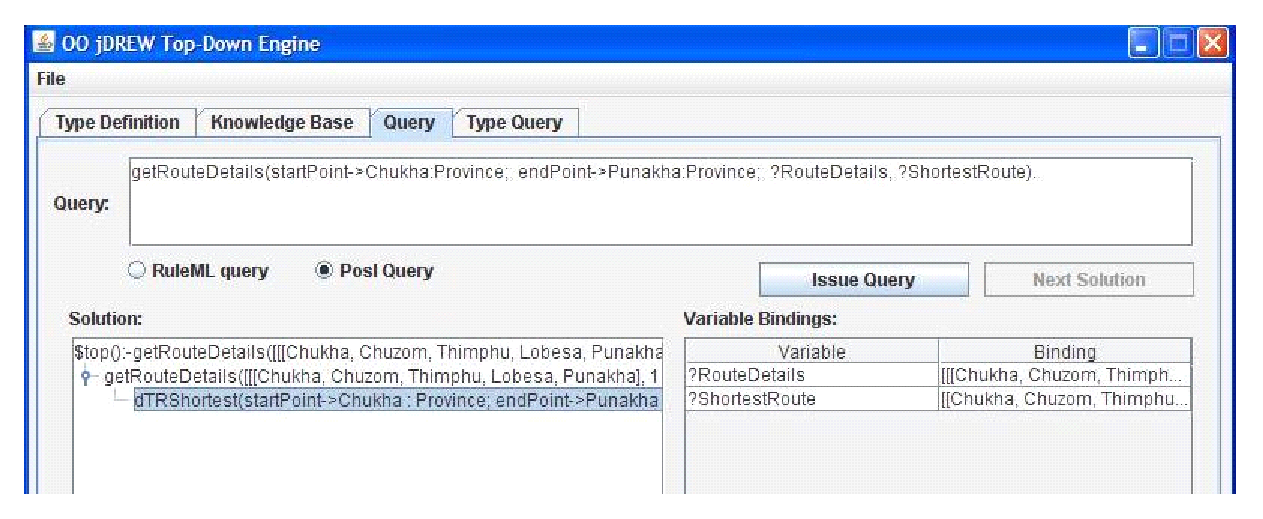
\includegraphics[width=6in]{Query1Table63}
\caption {Screenshot for Query 1 result}
\label{fig:Fig6.2}
\end{center}
\end{figure}

\subsubsection{Search for Activities}
\hspace{0.3in} The term ``Activity" subsumes both ``event" and ``attraction" classes introduced in Section 3.1. For each of the selected province profile of Bhutan, the fact base of our KB consists of stored FOAF-like profiles of attractions, events, and accommodations. These tourist entities are subclassified by the use of RDFS light-weight ontology type definitions (cf. Appendix E). The typed and well-formed KB offers a good powerful resource as a search engine to our users. Table 6.5 shows the different modes of searching for an activity. The systematic variation of these queries lies in the user's selected input slots.   

\begin{table} [tbph]
\caption{Queries of different input/output modes for Activity search}
\centering
\footnotesize
\begin{tabular}{|l|l|l|}
\hline
Query &\textbf{User Input} &$~~~~~~~~~~~~~~~~~~~~$ \textbf{Query Formats} \\
 &$~~$\textbf{Values}   & $~~~~~~~~~~~~$(Input values are bold-faced)      \\
\hline
 1&$~~$actName & getActivityDetails(actName-$>$\textbf{Paro\_Tshechu:Events};\\
  &        &$~~~~~~~~~~~~~~~~~~~~~~~~~$theme-$>?$Theme; \\
  &        &$~~~~~~~~~~~~~~~~~~~~~~~~~$address-$>?$Address; \\
  &        &$~~~~~~~~~~~~~~~~~~~~~~~~~?$ActivityDetails)\\
          
\hline
 2&$~~$actName:\emph{type}& getActivityDetails(actName-$>?$Name:\textbf{Festivals};\\
  &$~~~~$and/or      &$~~~~~~~~~~~~~~~~~~~~~~~~~$theme-$>?$Theme; \\
  & address element      &$~~~~~~~~~~~~~~~~~~~~~~~~~$address-$>$[?Subblock, \\
  &                       &$~~~~~~~~~~~~~~~~~~~~~~~~~~~~~~~~~~~~~~$\textbf{Chhoekhor:Block}, \\
  &                       &$~~~~~~~~~~~~~~~~~~~~~~~~~~~~~~~~~~~~~~?$Province,  \\
  &                       &$~~~~~~~~~~~~~~~~~~~~~~~~~~~~~~~~~~~~~~?$Region, \\
  &                       &$~~~~~~~~~~~~~~~~~~~~~~~~~~~~~~~~~~~~~~?$Country]; \\
  &                 &$~~~~~~~~~~~~~~~~~~~~~~~~~?$ActivityDetails)\\
          
\hline
 3&$~~~$theme & getActivityDetails(actName-$>?$Name;\\
  &$~~~~$and/or      &$~~~~~~~~~~~~~~~~~~~~~~~~~$theme-$>$\textbf{Cultural\_Religious\_Heritage}; \\
  & address element      &$~~~~~~~~~~~~~~~~~~~~~~~~~$address-$>$[?Subblock, \\
  &                       &$~~~~~~~~~~~~~~~~~~~~~~~~~~~~~~~~~~~~~~~?$Block, \\
  &                       &$~~~~~~~~~~~~~~~~~~~~~~~~~~~~~~~~~~~~~~~$\textbf{Paro:Province},\\
  &                       &$~~~~~~~~~~~~~~~~~~~~~~~~~~~~~~~~~~~~~~~?$Region, \\
  &                       &$~~~~~~~~~~~~~~~~~~~~~~~~~~~~~~~~~~~~~~~?$Country]; \\
  &                 &$~~~~~~~~~~~~~~~~~~~~~~~~~?$ActivityDetails)\\          
\hline 
 4&$~~~~$theme & getActivityDetails(actName-$>?$Name:\textbf{Events};\\
  &$~~~$actName:\emph{type}    &$~~~~~~~~~~~~~~~~~~~~~~~~~$theme-$>$\textbf{Recreation}; \\
  & address element      &$~~~~~~~~~~~~~~~~~~~~~~~~~$address-$>$[?Subblock, \\
  &                       &$~~~~~~~~~~~~~~~~~~~~~~~~~~~~~~~~~~~~~~~?$Block, \\
  &                       &$~~~~~~~~~~~~~~~~~~~~~~~~~~~~~~~~~~~~~~~?$Province,\\
  &                       &$~~~~~~~~~~~~~~~~~~~~~~~~~~~~~~~~~~~~~~~~$\textbf{Southern:Region}, \\
  &                       &$~~~~~~~~~~~~~~~~~~~~~~~~~~~~~~~~~~~~~~~?$Country]; \\
  &                 &$~~~~~~~~~~~~~~~~~~~~~~~~~?$ActivityDetails)\\        
 \hline
 5&$~~~~$None              & getActivityDetails(actName-$>?$Name;\\
  &    &$~~~~~~~~~~~~~~~~~~~~~~~~~$theme-$>$Theme; \\
  &       &$~~~~~~~~~~~~~~~~~~~~~~~~~$address-$>?$Address; \\
  &      &$~~~~~~~~~~~~~~~~~~~~~~~~~?$ActivityDetails)\\ 
\hline 
\end{tabular} 
\end{table}

\hspace{0.3in}The main options given to our users for searching an activity are primarily activity theme or type pertaining to a specific search area. The first option is useful if a user wants to retrieve more information about a specific event or attraction.
The ``type" relates to the RDFS type definition from the classfication of events and attractions collected from the Harmonise ontology (cf. Section 4.2). The type is attached to the activity name with a colon infix (`:'). 
This allows our users to make a more specific choice of the type of activity. The next input slot name, ``theme" is a broader sense of classification of the whole activity domain into three main themes, Cultural\_Religious\_Heritage, Nature, and Recreation. This classification of activity 
by theme is according to the Department of Tourism, Bhutan \cite{MZ:05}. Therefore, we allow users to search activities by either of the two classification or by specifying both. Query 4 in Table 6.5 is a good example, where users can get all activity details of type ``Events", belonging to the theme ``Recreation" in the ``Southern" region of the country. Query 5 is a special case where users specify nothing and the system binds the free slots to every activity profile in the KB. This is the most general form of querying compared to the most specific activity search in Query 4. To get a clear picture of the system output, we show the result to Query 4 in Table 6.6 (cf. the screenshot in Figure 6.4). The given solution is the only solution that meets the user's input specification for Query 4.

\begin{figure}
\begin{center}
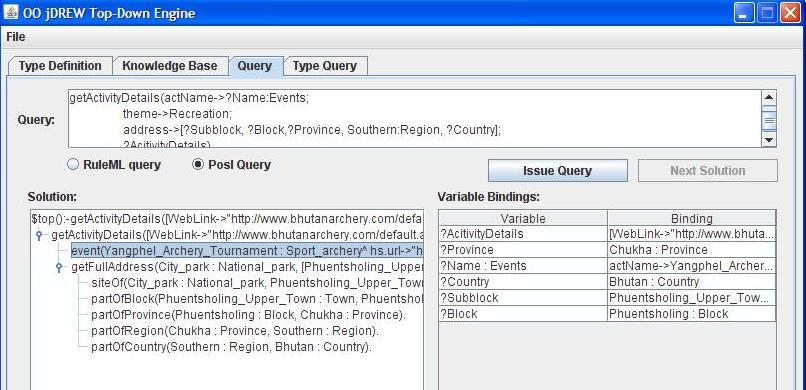
\includegraphics[width=6in]{Query4Table64}
\caption {Screenshot for Query 1 result}
\label{fig:Fig6.2}
\end{center}
\end{figure}


\begin{table} [tbph]
\caption{Activity search result of Query 4}
\centering
\footnotesize
\begin{tabular}{|l|l|}
\hline
 \textbf{Output} &$~~~~~~~~~~~~~~~~~~~~~~~~~~$\textbf{Variable Bindings} \\
 \textbf{Variables}&                \\
\hline
 $?$ActivityDetails&[ActName-$>$Yangphel\_Archery\_Tournament:Sport\_archery;\\
           &$~$WebLink-$>$``http://www.bhutanarchery.com/default.asp"; \\
		   &$~$EventDates-$>$[StartDate-$>$date[2008:Real, 08:Real, 23:Real];\\
           &$~~~~~~~~~~~~~~~~~~~~~$EndDate-$>$date[2008:Real, 10:Real, 02:Real]];\\	   
          &$~$Description-$>$``11TH Yangphel open archery tournament";\\
          &$~$Address-$>$[Phuentsholing\_Upper\_Town:Town, \\
		&$~~~~~~~~~~~~~~~~$Phuentsholing:Block, \\
		&$~~~~~~~~~~~~~~~~$Chukha:Province, \\
		&$~~~~~~~~~~~~~~~~$Southern:Region,\\
        &$~~~~~~~~~~~~~~~~$Bhutan:Country];\\
		&$~$Theme-$>$Recreation;\\
        &$~$RelatedTo-$>$``Thimphu\_Drupchen:Annual\_festival"] \\
 \hline
\end{tabular} 
\end{table}

\subsubsection{Search for Accommodations}
\hspace{0.3in}Similar to the activity search operations, the accommodation profiles structured with the RDFS light-weight ontology (described in Section 3.2) are used to provide users with some options for retrieving accommodation details for Bhutan. The main parameters for retrieving accommodation details are by name, type, price, or location. The systematic variation of queries are shown in Table 6.7.
\begin{table} [tbph]
\caption{Queries of different input/output modes for Accommodation search}
\centering
\footnotesize
\begin{tabular}{|l|l|l|}
\hline
 Query&\textbf{User Input} &$~~~~~~~~~~~~~~~~~~~~$ \textbf{Query Formats} \\
 &$~~$\textbf{Values}   &  $~~~~~~~~~~~~$(Input values are bold-faced)       \\
\hline
 1&$~~$accName & getAccommodationDetails(accName-$>$\textbf{Aman\_Resort:Resort};\\
  &        &$~~~~~~~~~~~~~~~~~~~~~~~~~~~~~~~~~~~~$address-$>?$Address; \\
  &        &$~~~~~~~~~~~~~~~~~~~~~~~~~~~~~~~~~~~~$setMaxPrice-$>?$SetMaxPrice; \\
  &        &$~~~~~~~~~~~~~~~~~~~~~~~~~~~~~~~~~~~?$AccommodationDetails)\\
\hline
 2&$~~$accName:\emph{type} & getAccommodationDetails(accName-$>?$Name:\textbf{Guest\_house};\\
  &$~~~~$and/or      &$~~~~~~~~~~~~~~~~~~~~~~~~~~~~~~~~~~~~$address-$>$[\textbf{Chamkhar:Town}, \\
  &address element     &$~~~~~~~~~~~~~~~~~~~~~~~~~~~~~~~~~~~~~~~~~~~~~~~~~~?$Block, \\
  &                       &$~~~~~~~~~~~~~~~~~~~~~~~~~~~~~~~~~~~~~~~~~~~~~~~~~~?$Province,  \\
  &                       &$~~~~~~~~~~~~~~~~~~~~~~~~~~~~~~~~~~~~~~~~~~~~~~~~~~?$Region, \\
  &                       &$~~~~~~~~~~~~~~~~~~~~~~~~~~~~~~~~~~~~~~~~~~~~~~~~~~?$Country]; \\ 
  &                       &$~~~~~~~~~~~~~~~~~~~~~~~~~~~~~~~~~~~~$setMaxPrice-$>?$SetMaxPrice;\\                
  &                      &$~~~~~~~~~~~~~~~~~~~~~~~~~~~~~~~~~~~?$AccommodationDetails)\\      
\hline
 3&$~~$setMaxPrice & getAccommodationDetails(accName-$>?$Name;\\
  &$~~~~$and/or      &$~~~~~~~~~~~~~~~~~~~~~~~~~~~~~~~~~~~~$address-$>$[\textbf{Chamkhar:Town}, \\
  &address element     &$~~~~~~~~~~~~~~~~~~~~~~~~~~~~~~~~~~~~~~~~~~~~~~~~~~?$Block, \\
  &                       &$~~~~~~~~~~~~~~~~~~~~~~~~~~~~~~~~~~~~~~~~~~~~~~~~~~?$Province,  \\
  &                       &$~~~~~~~~~~~~~~~~~~~~~~~~~~~~~~~~~~~~~~~~~~~~~~~~~~?$Region, \\
  &                       &$~~~~~~~~~~~~~~~~~~~~~~~~~~~~~~~~~~~~~~~~~~~~~~~~~~?$Country]; \\ 
  &                       &$~~~~~~~~~~~~~~~~~~~~~~~~~~~~~~~~~~~~$setMaxPrice-$>$[\textbf{Yes},\\
  &                       &$~~~~~~~~~~~~~~~~~~~~~~~~~~~~~~~~~~~~~~~~~~~~~~~~~~~~~~~~$\textbf{2000}:Real]; \\ 
  &                       &$~~~~~~~~~~~~~~~~~~~~~~~~~~~~~~~~~~~?$AccommodationDetails)\\
\hline
 4&$~~$accName:\emph{type} & getAccommodationDetails(accName-$>?$Name:\textbf{Resort};\\
  &$~~~$setMaxPrice      &$~~~~~~~~~~~~~~~~~~~~~~~~~~~~~~~~~~~~$address-$>$[\textbf{Tsento\_Shari:Village}, \\
  &address element      &$~~~~~~~~~~~~~~~~~~~~~~~~~~~~~~~~~~~~~~~~~~~~~~~~~~?$Block, \\
  &                       &$~~~~~~~~~~~~~~~~~~~~~~~~~~~~~~~~~~~~~~~~~~~~~~~~~~?$Province,  \\
  &                       &$~~~~~~~~~~~~~~~~~~~~~~~~~~~~~~~~~~~~~~~~~~~~~~~~~~?$Region, \\
  &                       &$~~~~~~~~~~~~~~~~~~~~~~~~~~~~~~~~~~~~~~~~~~~~~~~~~~?$Country]; \\ 
  &                       &$~~~~~~~~~~~~~~~~~~~~~~~~~~~~~~~~~~~~$setMaxPrice-$>$[\textbf{Yes},\\
  &                       &$~~~~~~~~~~~~~~~~~~~~~~~~~~~~~~~~~~~~~~~~~~~~~~~~~~~~~~~~$\textbf{1500}:Real]; \\ 
  &                       &$~~~~~~~~~~~~~~~~~~~~~~~~~~~~~~~~~~~?$AccommodationDetails)\\
\hline
 5&$~~~~$None & getAccommodationDetails(accName-$>?$Name;\\
  &        &$~~~~~~~~~~~~~~~~~~~~~~~~~~~~~~~~~~~~$address-$>?$Address; \\
  &        &$~~~~~~~~~~~~~~~~~~~~~~~~~~~~~~~~~~~~$setMaxPrice-$>?$SetMaxPrice; \\
  &        &$~~~~~~~~~~~~~~~~~~~~~~~~~~~~~~~~~~~?$AccommodationDetails)\\
\hline
\end{tabular} 
\end{table}

\hspace{0.3in} Accommodation information retrieval can be performed by name (i.e., the most specific), type, or user maximum affordable price (userMaxPrice) pertaining to a specific search area. Similar to what we have discussed earlier for province and activity search, Query 1 shows a mode of querying for accommodation by name. It is of interest to only users who want to retrieve the detailed information about a particular object of interest. The solution to this is always unique as names are the primary identifier of an entity in our KB. The input ``type" for the accommodation subdomain relates to the RDFS type definition of accommodation (cf. Section 4.2.3). We considered a simple type hierarchy for the accommodation consisting of only 4 main types, Guest\_house, Lodge, Hotel, and Resort (cf. Section 2.4). This allows our users to define a preference for the type of accommodation. Query 2 searches for a specfic type of accommodation pertaining to a specific part of the country. Another parameter to get accommodations is by a certain price bound within a specific search area (?Subblock, ?Block, ?Province, ?Region, ?Country). Query 3 retrieves two solutions as there are two accommodation profiles that are located in the subblock ``Chamkhar:Town" and does not cost more than ``2000 Ngultrum" (Ngultrum, Bhutanese currency). Then, in Query 4, we show a query which is specific about all the three options: type, userMaxPrice, and search area. There is only one solution that fulfills Query 4's specification (cf. the screenshot in Figure 6.5). The output variable bindings for this query are shown in Table 6.8. The last mode of query in Table 6.5 is the most general form of query (open query) where the free slots would be bound to every accommodation profile in the KB.\\


\begin{figure}
\begin{center}
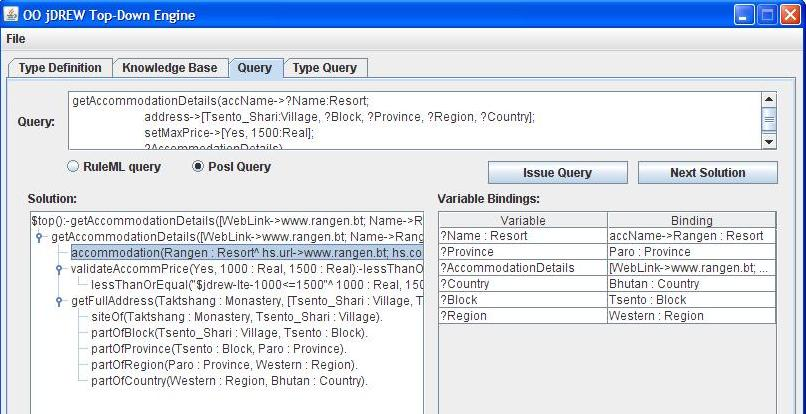
\includegraphics[width=6in]{Query4Table67}
\caption {Screenshot for Query 4 result}
\label{fig:Fig6.2}
\end{center}
\end{figure}

\begin{table} [tbph]
\caption{Accommodation search result of Query 4}
\centering
\footnotesize
\begin{tabular}{|l|l|}
\hline
 \textbf{Output} &$~~~~~~~~~~~~~~~~~~~~~~~$\textbf{Variable Bindings} \\
 \textbf{Variables}&                \\
\hline
 $?$AccommodationDetails&[AccName-$>$Rangen:Resort; \\
           &$~$WebLink-$>$``www.rangnen.bt "; \\
		    &$~$Address-$>$[Tsento\_Shari:Village, \\
		    &$~~~~~~~~~~~~~~~~$Tsento:Block, \\
		&$~~~~~~~~~~~~~~~~$Paro:Province, \\
		&$~~~~~~~~~~~~~~~~$Western:Region,\\
        &$~~~~~~~~~~~~~~~~$Bhutan:Country];\\
		   &$~$Standard-$>$[StarRating-$>$2:Real; \\
           &$~~~~~~~~~~~~~~~~~~$MinPrice-$>$1000:Real];\\
           &$~$ContactDetails-$>[$Telecoms-$>$[\\
            &$~~~~~~~~~~~~~~~~~~~~~~~~~~~~$Landline-$>$9758211452;\\
		        &$~~~~~~~~~~~~~~~~~~~~~~~~~~~~$Cell-$>$97517682948];\\
            &$~~~~~~~~~~~~~~~~~~~~~~~~~$Email-$>$"manager@rangen.bt"]; \\		   
          &$~$RelatedTo-$>$``Holiday\_Home:Hotel"];\\      
\hline
\end{tabular} 
\end{table} 
 
\subsubsection{Execution Times}
\hspace{0.3in}The experiments are performed in ITC 315, graduate student lab. The execution time is measured under Windows XP with Intel Core 2 Duo 2.66 GHz processor, 2.95 GB of RAM. The 00 jDREW engine version 0.96 is used on Eclipse platform with Java Runtime Environment version jre1.6.

\hspace{0.3in}The eTourPlan prototype, tested for a KB consisting of 73 facts and 37 rules, can perform any of the preceding search operations in reasonable time. The maximum time it takes for searching any of the tourist information is 4817 milliseconds. From our experiments, the engine takes longer time for open queries (all free slots) than for those with some fixed input (constants) from the user. Firing an open query forces the system to unify with all the facts as the query does not provide any specific unifying knowledge. On the other hand, for queries with some or all fixed arguments (constants), the engine instantly finds the exact match and returns the solution very fast.

\hspace{0.3in}The search performance of any of the preceeding subdomains are good due to two main reasons: 1) The object-centric profile descriptions of each of the subdomains are well-structured with RDFS type definitions and partonomy rules, which provides the flexibility to narrow down (or broaden) the search space. 2) Our search rules are object-centric and therefore search is localised to a specific domain.  

\subsection{Location-Centric Recommendation}

\hspace{0.3in}The location-centric recommender rule subsystem  has been described earlier (in Section 5.2.4). The eTourPlan prototype offers two main options, ``UserPrefBased" and ``SystemRecommendation". The two modes of querying for location-centric recommendations are shown in Table 6.9. For the first option, the system provides a simple recommendation of provinces and the routes between these provinces, which are selected by looking up in the FOAF relation between the provinces. This concept was described earlier for system route planning in Section 5.2.1.2. The user needs to provide the number of provinces and the starting province as shown in Query 1 in Table 6.9. The output from the system is a list of specified number of touristic provinces with some tourist information for each of the provinces. Tourist information includes the URL of the province, number of attractions, events, and accommodations for each of the provinces as shown in Table 6.10 (cf. the screenshot in Figure 6.6). It also provides the routes between these provinces. Similar concept is used for planning a travel in attraction-only mode, discussed in the next section.

\hspace{0.3in} Although our system-based recommendation provides good travel recommendation to our users, it is not enough for users who want to visit provinces of their own personal choice. This mode of querying for recommendation is described in the second row of Table 6.9. Users must provide their start and end point along with their preferred list of provinces to visit.  The system returns a list of tourist entities at each of the provinces along with routes between the selected provinces. The recommendation process collects all the events, attractions, and accommodations in each of the provinces and returns this accumulated list as the final solution. Sample output of the second mode of recommendation is shown in Table 6.11 (cf. the screenshot in Figure 6.7).

\begin{table} [tbph]
\caption{Queries of different input/output modes for Recommendation)}
\centering
\footnotesize
\begin{tabular}{|l|l|l|}
\hline
 &\textbf{User Input} &$~~~~~~~~~~~~~~~~~~~~$ \textbf{Query Formats} \\
 &$~~$\textbf{Values}   &$~~~~~~~~~~~~$(Input values are bold-faced)          \\
\hline
  1&typeOfRecommend & locCentricRecommend(typeOfRecommend-$>$\\
     &numProvinces        &$~~~~~~~~~~~~~~~~~~~~~~~~~~~~~~~~~$\textbf{SystemRecommendation};\\
     & &$~~~~~~$userInputs-$>$[startPoint-$>$\textbf{Paro:Province}; \\
     & &$~~~~~~~~~~~~~~~~~~~~$numProvinces-$>$\textbf{3}:Integer]; \\
         &                       &$~~~~~~$[$?$Routes, $?$Recommendations, $?$TotalBusHours]) \\          
\hline
 2&typeOfRecommend & locCentricRecommend(typeOfRecommend-$>$\textbf{UserPrefBased};\\
  &startPoint       &$~~~~~~$userInputs-$>$[startPoint-$>$\textbf{Paro:Province}; \\
  &userPrefList     &$~~~~~~~~~~~~~~~~~~~~~~~~$userPrefList-$>$\textbf{[Chukha:Province]};\\
  &endPoint         &$~~~~~~~~~~~~~~~~~~~~~~~~$endPoint-$>$\textbf{Thimphu:Province}]; \\
  &                       &$~~~~~~$[$?$Routes, $?$Recommendations, $?$TotalBusHours]) \\  
\hline      
\end{tabular} 
\end{table}

\begin{figure}
\begin{center}
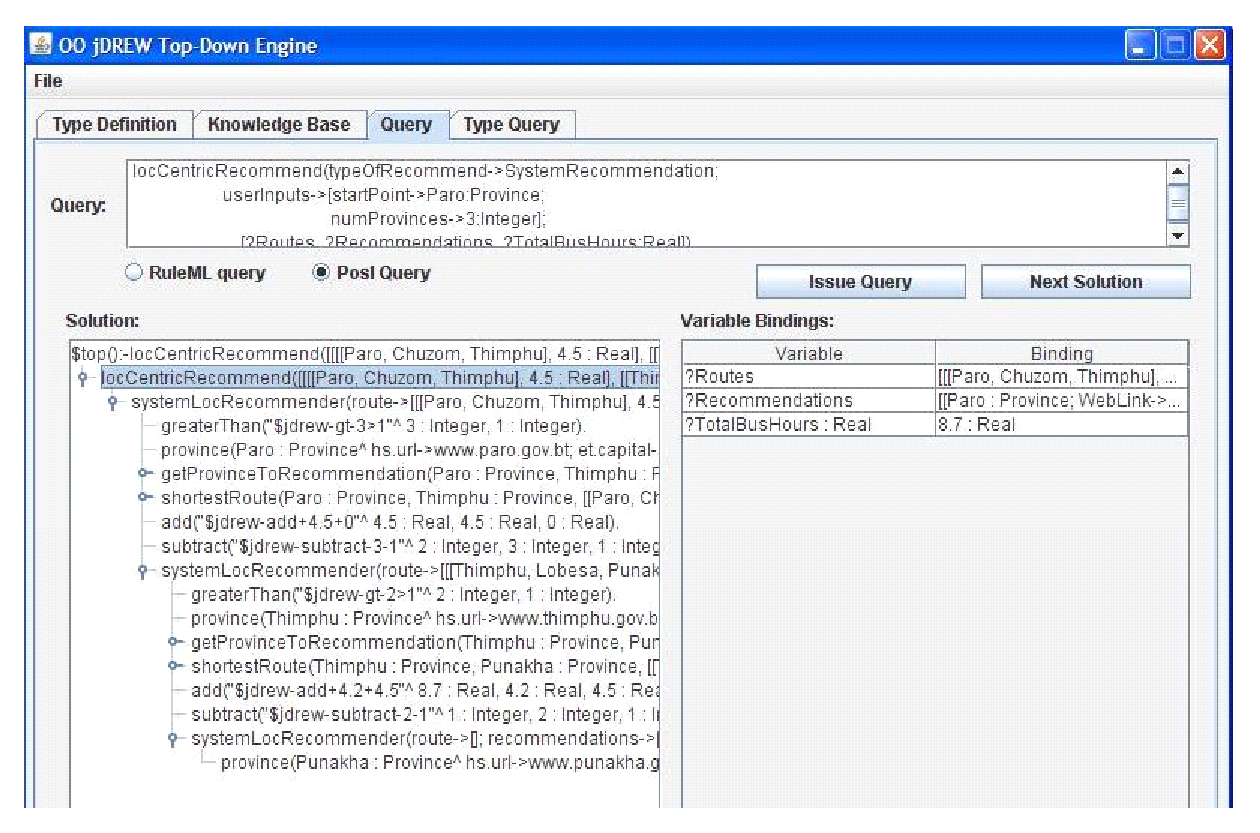
\includegraphics[width=6in]{LocSystem}
\caption {Screenshot for Test Query 1}
\label{fig:Fig6.4}
\end{center}
\end{figure}         


\begin{table} [tbph]
\caption{Location-centric recommendation by the system}
\centering
\footnotesize
\begin{tabular}{|l|l|}
\hline
 \textbf{Output} &$~~~~~~~~~~~~~~~~~~~~~~$\textbf{Variable Bindings} \\
 \textbf{Variables}&                \\
\hline
 $?$Routes  &[[Paro, Chuzom, Thimphu], 6.5 :Real],\\
           &$~$[[Thimphu, Lobesa, Punakha], 4.2:Real]]\\
 $?$Recommendations &[[Paro:Province;\\
  				    &$~~~~$WebLink-$>$``http://www.paro.gov.bt/"; \\
                   &$~~~~~~$TouristInfo-$>$\\
				   &$~~~~~~~~~$NumAttractions-$>$3:Integer; \\
		           &$~~~~~~~~~$NumEvents-$>$1:Integer; \\
			       &$~~~~~~~~~$NumAccommodations-$>$3:Integer]], \\
                   &$~$[Thimphu:Province; \\
  				    &$~~~~$WebLink-$>$``http://www.thimphu.gov.bt/"; \\
                   &$~~~~~~$TouristInfo-$>$\\
				   &$~~~~~~~~~$NumAttractions-$>$3:Integer; \\
		           &$~~~~~~~~~$NumEvents-$>$1:Integer; \\
			       &$~~~~~~~~~$NumAccommodations-$>$3:Integer]], \\
				   &$~$[Punakha:Province; \\
  				    &$~~~~$WebLink-$>$``http://www.punakha.gov.bt/"; \\
                   &$~~~~~~$TouristInfo-$>$\\
				   &$~~~~~~~~~$NumAttractions-$>$2:Integer; \\
		           &$~~~~~~~~~$NumEvents-$>$1:Integer; \\
			       &$~~~~~~~~~$NumAccommodations-$>$0:Integer]] \\
$?$TotalBusHours  &8.7:Real\\
\hline			   
\end{tabular} 
\end{table}         
\hspace{0.3in} In Query 2, the userPrefList is a singleton list with one province, ``Chukha". The recommender system accumulates all the attractions, events, and accommodation facilities. It also provides the shortest route from the starting point (Paro:Province) to the preferred location (Chukha:Province) and the shortest route from the last province in the user`s preference list to the specified end point (Thimphu:Province). 

\begin{figure}
\begin{center}
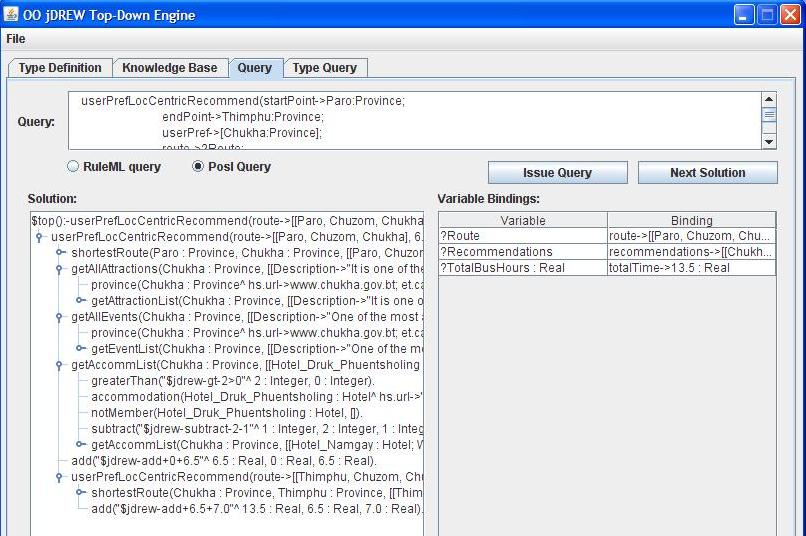
\includegraphics[width=6in]{LocUser}
\caption {Screenshot for Test Query 2}
\label{fig:Fig6.4}
\end{center}
\end{figure}         
\begin{table} [tbph]
\caption{Location-centric recommendation for user-preferred Provinces}
\centering
\footnotesize
\begin{tabular}{|l|l|}
\hline
 \textbf{Output} &$~~~~~~~~~~~~~~~~~~~~~~~~~~$\textbf{Variable Bindings} \\
 \textbf{Variables}&                \\
\hline
 $?$Routes  &[[Paro, Chuzom, Chukha], 6.5 :Real,\\
           &$~$[Chukha, Chuzom, Thimphu], 7.0 :Real]\\
 $?$Recommendations&[Chukha; \\
                   &EventList-$>$\\
  				   &$~~~~$[[EventName-$>$Chukha\_Tshechu:Annual\_festival;\\
				   &$~~~~~~$Description-$>$``One of the most amazing festivals in Chukha";\\
				   &$~~~~~~$Address-$>$[Chukha\_Town:Town, \\
		           &$~~~~~~~~~~~~~~~~~~~~$Gelling:Block, \\
		           &$~~~~~~~~~~~~~~~~~~~~$Southern:Region, \\
		           &$~~~~~~~~~~~~~~~~~~~~$Bhutan:Country,\\
                 &$~~~~~~$EventDates-$>$[StartDate-$>$date[2008:Real, 03:Real, 19:Real];\\
                &$~~~~~~~~~~~~~~~~~~~~~~~~~$EndDate-$>$date[2008:Real, 03:Real, 21:Real]]],\\	   
                  &$~~~~~$[EventName-$>$Yangphel\_Archery\_Tournament:Sport\_archery;\\
				   &$~~~~~~$Description-$>$``11TH Yangphel open archery tournament";\\
				   &$~~~~~~$Address-$>$[Phuentsholing\_Upper\_Town:Town, \\
		         &$~~~~~~~~~~~~~~~~~~~~$Phuentsholing:Block,, \\
		          &$~~~~~~~~~~~~~~~~~~~~$Southern:Region, \\
		           &$~~~~~~~~~~~~~~~~~~~~$Bhutan :Country,\\
                 &$~~~~~~$EventDates-$>$[StartDate-$>$date[2008:Real, 08:Real, 23:Real];\\
             &$~~~~~~~~~~~~~~~~~~~~~~~~~$EndDate-$>$date[2008:Real, 10:Real, 02 :Real]]]]; \\	     
		   &AttractionList-$>$\\
  				   &$~~~~$[[AttractionName-$>$Chukha\_Dzong:Fortress;\\
				   &$~~~~~~$WebLink-$>$`` "; \\
				   &$~~~~~~$Description-$>$``It is one of the most beautiful attractions.";\\
				   &$~~~~~~$Address-$>$[Chukha\_Town:Town, \\
		          &$~~~~~~~~~~~~~~~~~~~~$Gelling:Block, \\
		           &$~~~~~~~~~~~~~~~~~~~~$Southern:Region, \\
		           &$~~~~~~~~~~~~~~~~~~~~$Bhutan :Country,\\
				   &$~~~~~~$Theme-$>$Cultural\_Religious\_Heritage;\\
          
		   &AccommodationList-$>$\\
  				   &$~~~~$[[Hotel\_Druk\_Phuentsholing:Hotel; \\
			       &$~~~~~~$WebLink-$>$``www.drukhotels.com/"; \\
                   &$~~~~~~$MinPrice-$>$"2700:Real";\\
				   &$~~~~~~$Rating-$>$4:Real], \\
		           &$~~~~$[Hotel\_Namgay:Hotel;  \\
			       &$~~~~~~$WebLink-$>$``www.hotelNamgay.bt/"; \\
                   &$~~~~~~$MinPrice-$>$"1800:Real";\\
				   &$~~~~~~$Rating-$>$3:Real]]]] \\	
\hline				   
$?$TotalBusHours  &13.5:Real\\
\hline			   
\end{tabular} 
\end{table} 
       
 
\subsubsection{Execution Times}
\hspace{0.3in}The execution of Query 1 and Query 2 (cf. Table 6.9) takes 16218 and 1523781 milliseconds, respectively. As we can see in the outputs of the two modes of operations, the location-centric recommendation for user-preferred provinces (Query 2) takes comparatively large amount of time to system recommendation of provinces (Query 1). This is because it is only in the second mode of recommendation that we integrate ``getAllAttractions", ``getAllEvents", and ``getAllAccommodations" recursive predicates. For each recursive predicate, as the number of iteration increases from 1 to N, the execution time gets exponentially high. Another source of inefficiency is from the fact that the textual order between rule is not exploited by our pure logic programs, thereby performing unnecessary searches for candidate bindings. %The negative subpredicate ``notMember" is used to avoid revisitation or duplicates in the result. 

\subsection{Complete Travel Planning Operation}
 
\hspace{0.3in} We will now look at different scenarios of planning and the corresponding output results. eTourPlan offers two main planning options, ``Attractions-only" and ``Event-centric", as shown in Table 6.12. 
\subsubsection{Attraction-Only Planning}
\hspace{0.3in}The first option for travel planning is the attraction-based planning. It uses the FOAF relation between attractions similar to related provinces in location-centric planning. Users has to input the starting point, the number of attractions and the total trip time in days. The system accumulates the FOAF-related attractions from the given starting province and chains along until it finds the specified number of N attractions for the user.
The output variable ``?TravelResult" binds to a detailed attraction list, whicn includes route
information as well. Currently, the routes are implemented only between provinces. However, the route computation can be done at a finer granularity, at the subblock level for provinces, by applying the same route computation approach. The last output argument in the list that binds to ``?TravelResult" is the ?TotalActivityTimeInHours. This is the sum of the route hours and the total of ``?MaxHoursAtAnAttractionSite" for N attractions. A screenshot of the eTourPlan ``Attraction0nly" planning 
is shown in Figure 6.8. The resulting output variable bindings shown in Table 6.13 describe the travel result. The result is a trip scheduled for visiting 4 attractions (two fortresses, a monastery and a national museum). It provides the important details, such as the URL, description, theme, opening hours, and location for each attraction selected through the FOAF relations of attraction profiles. It also provides the provincial route information between the provinces. The total time (includes both travel and activity hours) for the entire trip is also computed.

\begin{table} [tbph]
\caption{Queries of different input/output modes for Travel Planning}
\centering
\footnotesize
\begin{tabular}{|l|l|l|}
\hline
 &\textbf{User Input} &$~~~~~~~~~~~~~~~~~~~~$ \textbf{Query Formats} \\
 &$~~$\textbf{Values}   & $~~~~~~~~~~~~$(Input values are bold-faced)   \\
\hline
 1&typeOfPlanning &eTourPlan(typeOfPlanning-$>$\textbf{AttractionOnly};\\
  &startPoint     &$~~~$userInputs-$>$[startPoint-$>$\textbf{Paro:Province}; \\
  &endPoint         &$~~~~~~~~~~~~~~~~~~~~$endPoint-$>$\textbf{Thimphu:Province}; \\
  &numAttractions   &$~~~~~~~~~~~~~~~~~~~~$numAttractions-$>$\textbf{4}:Integer;\\ &userTotalTravelTimeInDays&$~~~~~~~~~~~~~~~~~~~$userTotalTravelTimeInDays-$>$\textbf{4}:Integer];\\
  &                       &$~~~?$TravelResult) \\        
\hline
2&typeOfPlanning & eTourPlan(typeOfPlanning-$>$\textbf{EventCentric};\\
   &                        &$~$userInputs-$>$[\\
   &startPoint          &$~~~$startPoint-$>$\textbf{Paro:Province}; \\
  &endPoint       &$~~~$endPoint-$>$\textbf{Thimphu:Province}; \\
  &userStartDate  &$~~~$userStartDate-$>$\textbf{date[2008:Real,10:Real,01:Real]}; \\
  &userEndDate    &$~~~$userEndDate-$>$\textbf{date[2008:Real,11:Real,10:Real]}; \\
  &maxBreak       &$~~~$maxBreak-$>$\textbf{10:Real}; \\
  &minBreak       &$~~~$minBreak-$>$\textbf{0:Real}; \\
  &attractionRecommendation&$~~~$attractionRecommendation-$>$\textbf{No}; \\
  &eventNum      &$~~~$eventNum-$>$\textbf{2:Integer}]; \\
  &                      &$~?$TravelResult)\\         
\hline
\end{tabular} 
\end{table}

\begin{figure}
\begin{center}
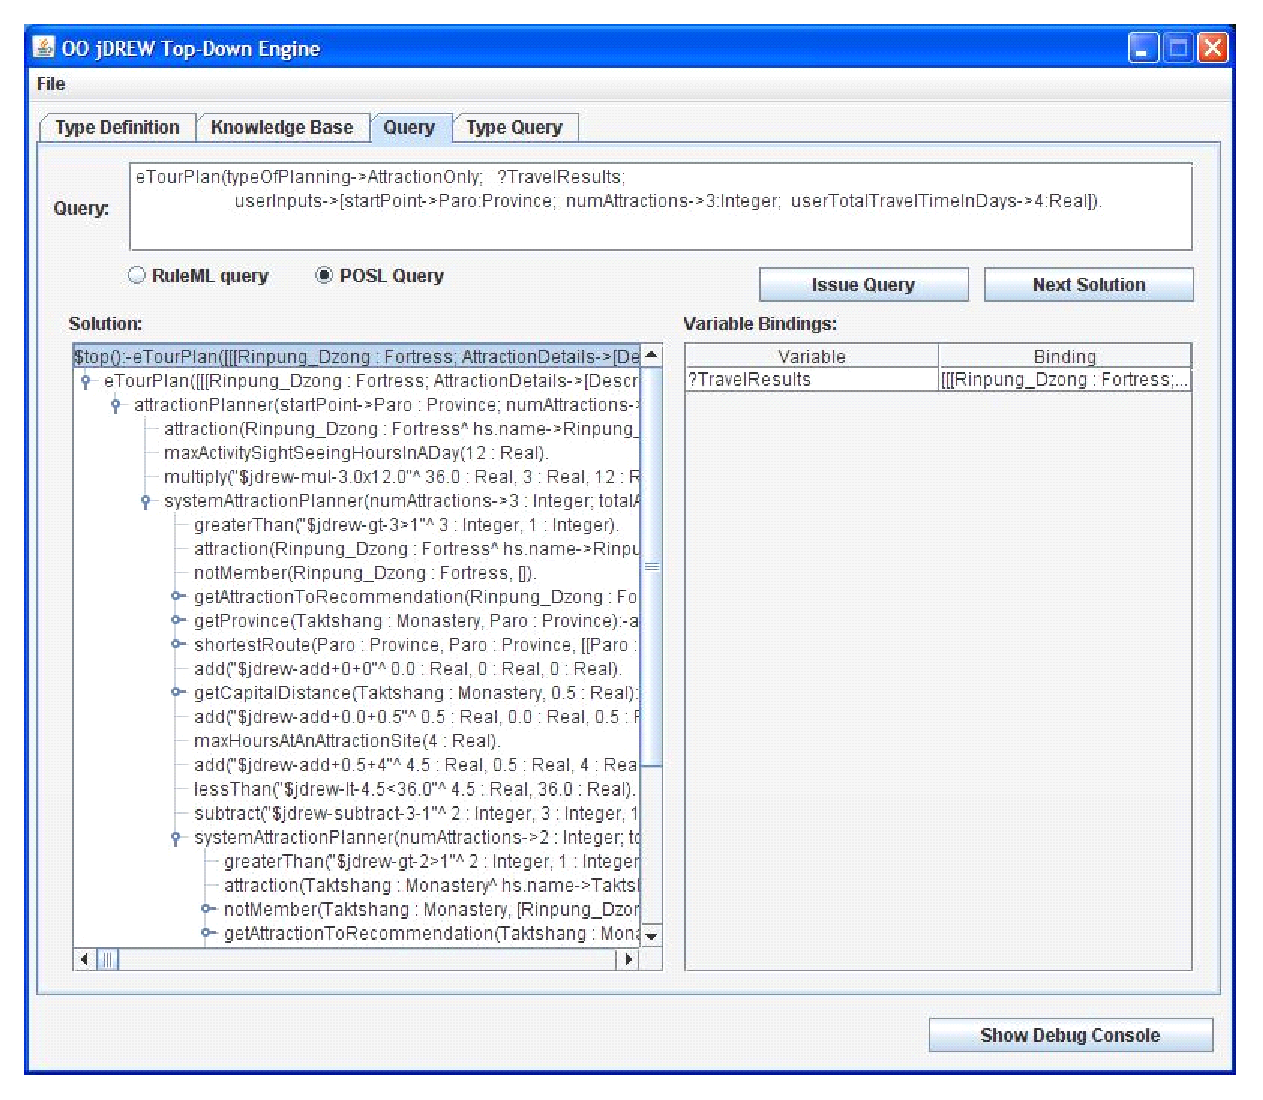
\includegraphics[width=6in]{screenshotAttraction}
\caption {Screenshot for Querying ``AttractionOnly" travel}
\label{fig:Fig6.3}
\end{center}
\end{figure}


\begin{table} [tbph]
\caption{Attraction-only travel result}
\centering
\footnotesize
\begin{tabular}{|l|l|}
\hline
 \textbf{Output} &$~~~~~~~~~~~~~~~~~~~~~~~~~~$\textbf{Variable Bindings} \\
 \textbf{Variables}&                \\
\hline
 $?$TravelResult&\cellcolor{yellow}[Name-$>$Rinpung\_Dzong:Fortress;\\
  		 &$~$AttractionDetails-$>$[ \\
  		 &$~~~$Url-$>$`` ";	\\
		    &$~~~$Description-$>$``It is one of the most beautiful";\\
			  &$~~~~~~~~~~~~~~~~~~~~~~$attractions in the Western region.";\\
			  &$~~~$Theme-$>$Cultural\_Religious\_Heritage;\\
			  &$~~~$OpenHours-$>$Open[DaysOfWeek[Mon,Tue,Wed,Thu,Fri,Sat,Sun],\\
		  	&$~~~~~~~~~~~~~~~~~~~~~$Period[9:Real, 16:Real]];\\
			&$~~~$Location-$>$[Phatsana:Village, Paro:Province]];\\
			&$~~~$Route-$>$[[Paro:Province], 0:Real],\\
       &\cellcolor{yellow}[Name-$>$Taktshang:Monastery;\\
  		 &$~$AttractionDetails-$>$[ \\
  		 &$~~~$Url-$>$`` ";	\\
		    &$~~~$Description-$>$``It is known as the tiger's Nest,;\\
			  &$~~~~~~~~~~~~~~~~~~~~~~$one of the seven wonders of in the world.";\\
			  &$~~~$Theme-$>$Cultural\_Religious\_Heritage;\\
			  &$~~~$OpenHours-$>$Open[DaysOfWeek[Mon,Tue,Wed,Thu,Fri,Sat,Sun],\\
		  	&$~~~~~~~~~~~~~~~~~~~~~$Period[8:Real, 18:Real]];\\
			&$~~~$Location-$>$[Tshento\_Shari:Village, Paro:Province]];\\
			&$~~~$Route-$>$[[Paro:Province], 0:Real],\\
			&\cellcolor{yellow}[Name-$>$Ta\_Dzong: National\_museum;\\
  		 &$~$AttractionDetails-$>$[ \\
  		 &$~~~$Url-$>$``www.nationalmuseum.gov.bt";	\\
		    &$~~~$Description-$>$"It is the biggest and the oldest;\\
			  &$~~~~~~~~~~~~~~~~~~~~~~$museum in Bhutan";\\
			  &$~~~$Theme-$>$Cultural\_Religious\_Heritage;\\
			  &$~~~$OpenHours-$>$Open[DaysOfWeek[Tue,Wed,Thu,Fri,Sat,Sun],\\
		  	&$~~~~~~~~~~~~~~~~~~~~~$Period[10:Real, 16:Real]];\\
			&$~~~$Location-$>$[Goepay:Village, Paro:Province]];\\
			&$~~~$Route-$>$[[Paro, Thimphu], 4.5:Real]],\\   
      &\cellcolor{yellow}[Name-$>$Tashichoe\_Dzong:Fortress;\\
  		 &$~$AttractionDetails-$>$[ \\
  		 &$~~~$Url-$>$`` ";	\\
		 &$~~~$Description-$>$``It is one of the most beautiful;\\
			  &$~~~~~~~~~~~~~~~~~~~~~~$attractions in the Capital";\\
			  &$~~~$Theme-$>$Cultural\_Religious\_Heritage;\\
			  &$~~~$OpenHours-$>$Open[DaysOfWeek[Tue,Wed,Thu,Fri,Sat,Sun],\\
		  	&$~~~~~~~~~~~~~~~~~~~~~$Period[9:Real, 16:Real]];\\
			&$~~~$Location-$>$[Jongshina:Town, Thimphu:Province]];\\
			&$~~~$Route-$>$[[Thimphu:Province], 0:Real]]];\\
		 &$~~~$	\\
	 &TotalActivityTimeInHours-$>$22.5: Real\\   
\hline		   
\end{tabular} 
\end{table} 

\begin{table} [tbph]
\caption{Execution times for Attraction-only Planning}
\centering
\footnotesize
\begin{tabular}{|l|l|}
\hline
  ?NumAttractions:Integer & Execution Times (in Milliseconds)\\
\hline
  1  & 250 \\
\hline
  2   &18812 \\
\hline
  3 & 313250\\
\hline
  4 & 3453297 \\
\hline
\end{tabular} 
\end{table} 

\subsubsection{Scenarios of Event Planning}
\hspace{0.3in}eTourPlan's event-centric planning is the primary operation that integrates the other rule subsystems (cf. Figure 6.1). The event planner handles the event scheduling with respect to event schedules and distances between event locations for a user-specified travel dates. The planner provides attraction recommendations at the subblocks of the event locations. It also provides an additional option of on-route attraction recommendations between event locations, considering the possibility of a big time gap between two events. This optimises the resulting travel output to users incase there is only one event within the user-specified dates and it has a long route to the event location. User can either check ``Yes" or ``No" to this option. We will now look at some examples of querying the eTourPlan event-centric planner with varying test queries. 

\hspace{0.3in}\textbf{Example 1}:\emph{User queries for an event-centric plan of 1 events between the 1st of
October and the 10th of November and specifies a ``maxBreak" of 10
days and ``minBreak" of 0 days between main events. User also
specifies the starting province, ``Paro:Province", and the final
destination province, as ``Thimphu:Province". User checks ``No" for
on-route attraction recommendation, knowing that the planner
provides recommendation of attractions at the subblock of event
location.}\\

\hspace{0.3in}\textbf{Test Query 1}:

\begin{small}
\singlespacing
\begin{verbatim}
 eTourPlan(typeOfPlanning->EventCentric;  
           ?TravelResult;
           userInputs->[userStartDate->date[2008:Real, 11:Real, 01:Real];  
                        userEndDate->date[2008:Real, 11:Real, 04:Real]; 
                        maxBreak->4:Real;  
                        minBreak->0:Real; 
                        startPoint->Paro:Province;  
                        endPoin->Thimphu:Province;
                        attractionRecommendation->No; 
                        eventNum->1:Integer]).
\end{verbatim}
\end{small}

\hspace{0.3in} The system returns ``No solution" since there is no successful binding to this query, meaning the system fails to find any event in the KB that is occuring between the above dates.\\  

\hspace{0.3in}\textbf{Example 2}:\emph{User queries for an event-centric plan of 2 events between the 1st of October and the 10th of November. The user specifies a ``maxBreak" of 10 days and ``minBreak" of 0 days between main events.
User specifies the starting province,``Paro: Province", and the final
destination province, as ``Thimphu:Province". The user selects ``No" for
on-route attraction recommendation, knowing that the planner
provides recommendation of attractions at the subblock of event
location.}\\

\hspace{0.3in}\textbf{Test Query 2}:
\begin{small}
\singlespacing
\begin{verbatim}
 eTourPlan(typeOfPlanning->EventCentric; ?TravelResult;
           userInputs->[userStartDate->date[2008:Real, 10:Real, 01:Real];  
                        userEndDate->date[2008:Real, 11:Real, 10:Real]; 
                        maxBreak->10:Real;  
                        minBreak->0:Real; 
                        startPoint->Paro:Province;  
                        endPoin->Thimphu:Province;
                        attractionRecommendation->No; 
                        eventNum->2:Integer]).
\end{verbatim} 
\end{small}

\hspace{0.3in}The system returns 6 alternative solutions to this query. There are 5 events occuring between the user-specified time interval. The planner takes care of time and distance constraint validation, resulting in selective combinations of events. The Screenshots showing the first two test results for this query are shown in Figures 6.9 and 6.10. The selected event combinations in the output are recorded in Table 6.16. The second column contains the list of all events that are found within the user's specified trip dates. The third column corresponds to each of the event combinations generated by the system. For example, the first result generated by the system selects event 1 (Tamshingphala\_Choepa:Traditional\_festival) and event 2 (Tangbi\_Mani:Traditional\_festival), which are both located in Bumthang province and validated with user's time specification for a travel. The complete output variable bindings shown in Table 6.15 describe the travel result. It provides important details, such as the URL, description, theme, event dates, and location for each selected event. It also provides recommendation of attractions sited at the event-occuring subblock and the provincial route information between the provinces. 

\begin{table} [tbph]
\caption{Event-Centric travel results}
\centering
\footnotesize
\begin{tabular}{|l|l|}
\hline
 \textbf{Output} &$~~~~~~~~~~~~~~~~~~~~~~~~~~$\textbf{Variable Bindings} \\
 \textbf{Variables}&                \\
\hline
 $?$TravelResult&\cellcolor{yellow}[[[EventName-$>$Tamshingphala\_Choepa:Traditional\_festival;\\
  		 &$~~$EventDates-$>$[Startdate-$>$date[2008:Real, 10:Real, 08:Real];\\
		    &$~~~~~~~~~~~~~~~~~~~~~$Enddate-$>$date[2008:Real, 10:Real, 10:Real]];\\
			  &$~~$Theme-$>$Cultural\_Religious\_Heritage;\\
			  &$~~$EventDescription-$>$``One of the most amazing festivals in Bumthang"\\
		  	  &$~~$Location-$>$[Tamshing\_Lhakhang:Temple, \\
		  	  &$~~~~~~~~~~~~~~~~~$Tamshing\_Village:Village,\\ 
		  	  &$~~~~~~~~~~~~~~~~~$Bumthang:Province];\\
			  &$~~$RelatedEvent-$>$Tangbi\_Mani:Traditional\_festival;\\
			&$~~${\color{blue}RouteDetails}-$>$[[Paro:Province, Chuzom:Province, Thimphu:Province,\\
      &$~~~~~~~~~~~~~~~~~~~~~~~~$Lobesa:Province, WangduePhodrang:Province, \\ 
			&$~~~~~~~~~~~~~~~~~~~~~~~~$Trongsa:Province, Bumthang:Province], \\
			&$~~~~~~~~~~~~~~~~~~~~~~~~$[]; RouteBusHours-$>$16.7:Real];\\
						
		   &$~~${\color{blue}RecommendedAttractions}-$>$[Tamshing\_Lhakhang:Temple, \\
		   &$~~~~~~~$``It was built by Pema Lingpa,the Treasure Revealer in 1505."]],\\
         &$~~$\cellcolor{yellow}[EventName-$>$Tangbi\_Mani:Traditional\_festival;\\
  		 &$~~$EventDates-$>$[Startdate-$>$date[2008:Real, 10:Real, 13:Real;\\
		    &$~~~~~~~~~~~~~~~~~~~~~$Enddate-$>$date[2008:Real, 10:Real, 15:Real]];\\
			  &$~~$Theme-$>$Cultural\_Religious\_Heritage;\\
			  &$~~$EventDescription-$>$``A prestigious annual festival in Bumthang"\\
		  	  &$~~$Location-$>$[Tangbi\_Monastery:Monastery, \\
		  	  &$~~~~~~~~~~~~~~~~~$Tangbi:Village,\\ 
		  	  &$~~~~~~~~~~~~~~~~~$Bumthang:Province];\\
			  &$~~$RelatedEvent-$>$Wangdue\_Tshechu:Annual\_festival; \\
			&$~~${\color{blue}RouteDetails}-$>$[Bumthang:Province],  \\
      &$~~~~~~~~~~~~~~~~~~~~~~~$[]; RouteBusHours-$>$0:Real]]]; \\ 
									
		   &$~~${\color{blue}RecommendedAttraction}-$>$[Tangbi\_Monastery:Monastery \\
		   &$~~~~~~~$``Located in upper Tang valley."]],\\	   
       &$~~${\color{blue}ReturnRoute}-$>$[[Bumthang:Province, Trongsa:Province,  \\   
	   &$~~~~~~~~~~~~~~~~~~~~~~$WangduePhodrang:Province,Lobesa:Province, \\
	   &$~~~~~~~~~~~~~~~~~~~~~~$Thimphu:Province]; Returntime-$>$12.2:Real]]\\
\hline		   
\end{tabular} 
\end{table} 

\begin{table} [tbph]
\caption{Evaluation of event-centric travel results}
\centering
\footnotesize
\begin{tabular}{|l|l|l|}
\hline
Event &Event Schedules &Event Sequences\\
 & & $~~~~~$of length\\
 & &$~$ ?EventNum= 2\\
 \hline
  1  &Tamshingphala\_Choepa:Traditional\_festival&\textbf{1,2}\\
     &startDate-$>$date[2008:Real,10:Real,08:Real]&\textbf{1,5}\\
   &endDate-$>$date[2008:Real,10:Real,10:Real]&\\
   &province-$>$Bumthang&\\
\hline
  2  &Tangbi\_Mani:Traditional\_festival&\\
     &startDate-$>$date[2008:Real,10:Real,13:Real]&\\
   &endDate-$>$date[2008:Real,10:Real,15:Real]&\\
   &province-$>$Bumthang&\\
\hline
  3  &Thimphu\_Drupchen:Annual\_festival&\textbf{3,2}\\
     &startDate-$>$date[2008:Real,10:Real,04:Real]&\textbf{3,4}\\
   &endDate-$>$date[2008:Real,10:Real,08:Real]&\\
   &province-$>$Thimphu&\\
\hline
 4  &Thimphu\_Tshechu:Annual\_festival&\textbf{4,2}\\
     &startDate-$>$date[2008:Real,10:Real,09:Real]&\textbf{4,5}\\
   &endDate-$>$date[2008:Real,10:Real,11:Real]&\\
   &province-$>$Thimphu&\\
\hline
 5  &Wangdue\_Tshechu:Annual\_festival&\\
     &startDate-$>$date[2008:Real,10:Real,20:Real]&\\
   &endDate-$>$date[2008:Real, 10:Real, 29:Real]&\\
   &province-$>$WangduePhodrang&\\
\hline
\end{tabular} 
\end{table}  

\hspace{0.3in}The results in column 3 (Table 6.17) are shown are in the order of executed results in OO jDREW TD. The highlighted area of the trace in the output Screenshot (cf. Figure 6.9) shows the next selected event. 

\begin{table} [tbph]
\caption{Evaluation of event-centric travel results}
\centering
\footnotesize
\begin{tabular}{|l|l|l|}
\hline
Event &Event Schedules &Event Sequences\\
 & & $~~~~~$of length\\
 & &$~$ ?EventNum= 3\\
\hline
  1  &Tamshingphala\_Choepa:Traditional\_festival&\textbf{1,2,5}\\
     &startDate-$>$date[2008:Real,10:Real,08:Real]&\\
   &endDate-$>$date[2008:Real,10:Real,10:Real]&\\
   &province-$>$Bumthang&\\
\hline
  2  &Tangbi\_Mani:Traditional\_festival&\\
     &startDate-$>$date[2008:Real,10:Real,13:Real]&\\
   &endDate-$>$date[2008:Real,10:Real,15:Real]&\\
   &province-$>$Bumthang&\\
\hline
  3  &Thimphu\_Drupchen:Annual\_festival&\textbf{3,2,5}\\
     &startDate-$>$date[2008:Real,10:Real,04:Real]&\textbf{3,4,2}\\
   &endDate-$>$date[2008:Real,10:Real,08:Real]&\textbf{3,4,5}\\
   &province-$>$Thimphu&\\
\hline
 4  &Thimphu\_Tshechu:Annual\_festival&\textbf{4,2,5}\\
     &startDate-$>$date[2008:Real,10:Real,09:Real]&\\
   &endDate-$>$date[2008:Real,10:Real,11:Real]&\\
   &province-$>$Thimphu&\\
\hline
 5  &Wangdue\_Tshechu:Annual\_festival&\\
     &startDate-$>$date[2008:Real,10:Real,20:Real]&\\
   &endDate-$>$date[2008:Real, 10:Real, 29:Real]&\\
   &province-$>$WangduePhodrang&\\
\hline
\end{tabular} 
\end{table} 


\begin{figure}
\begin{center}
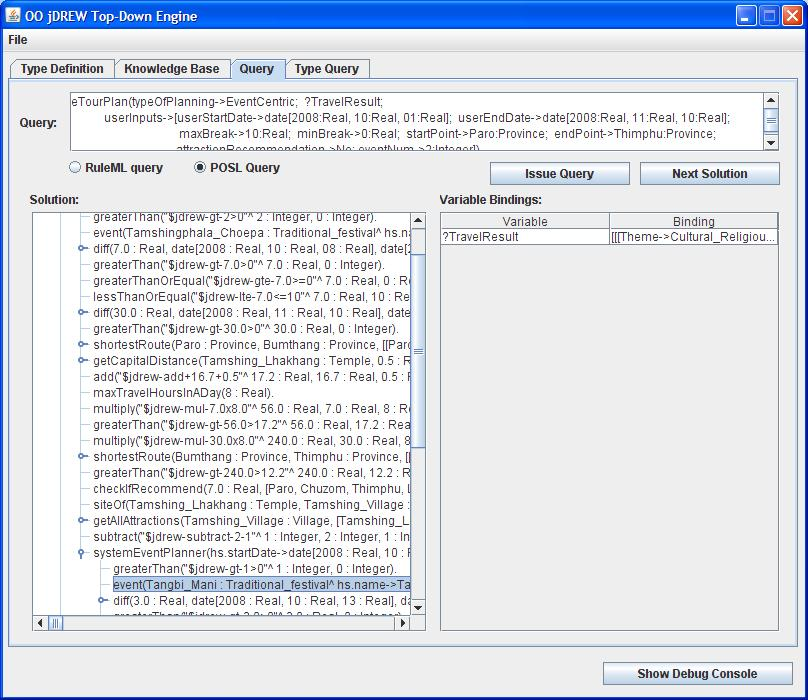
\includegraphics[width=6in]{2EP1}
\caption {Screenshot for Test Query 2, First Solution}
\label{fig:Fig6.3}
\end{center}
\end{figure}

\begin{figure}
\begin{center}
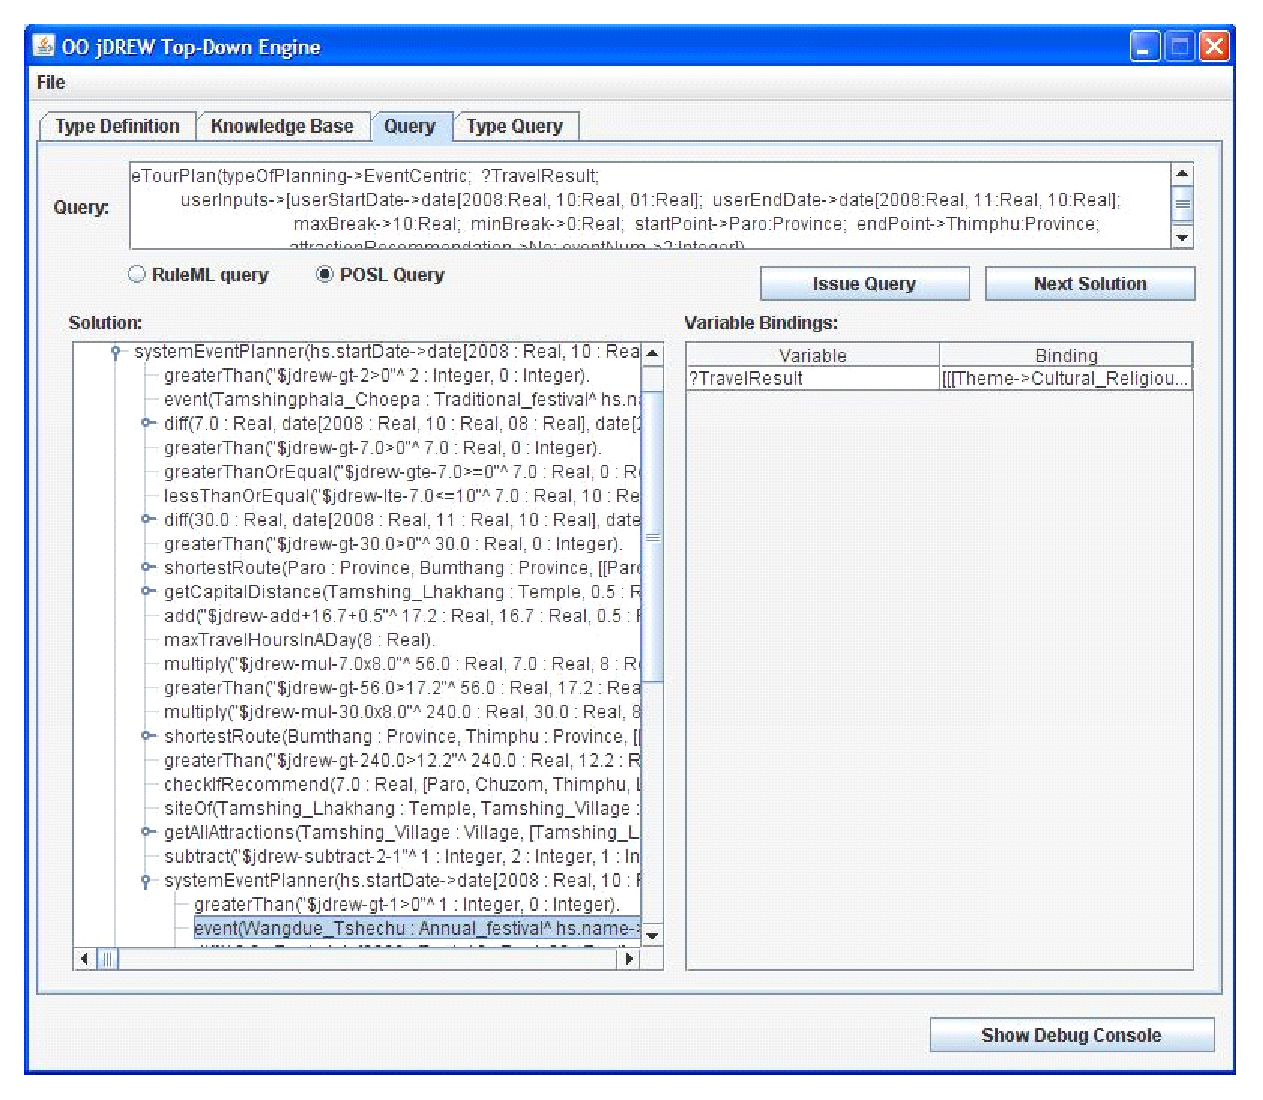
\includegraphics[width=6in]{2EP2}
\caption {Screenshot for Test Query 2, Next Solution}
\label{fig:Fig6.3}
\end{center}
\end{figure}
%\begin{figure}
%\begin{center}
%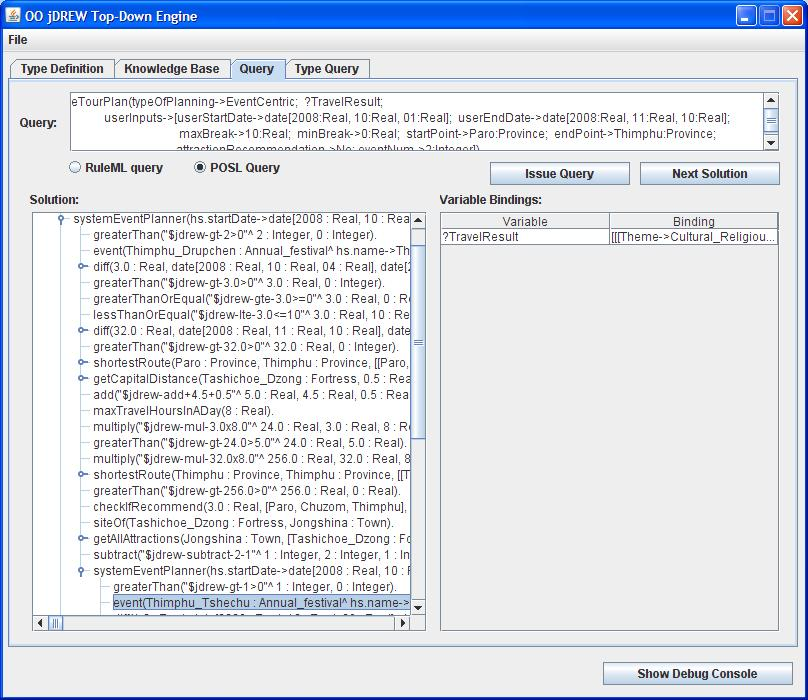
\includegraphics[width=6in]{2EP3}
%\caption {Screenshot for Test Query 2, Next Solution}
%\label{fig:Fig6.3}
%\end{center}
%\end{figure}

%\begin{figure}
%\begin{center}
%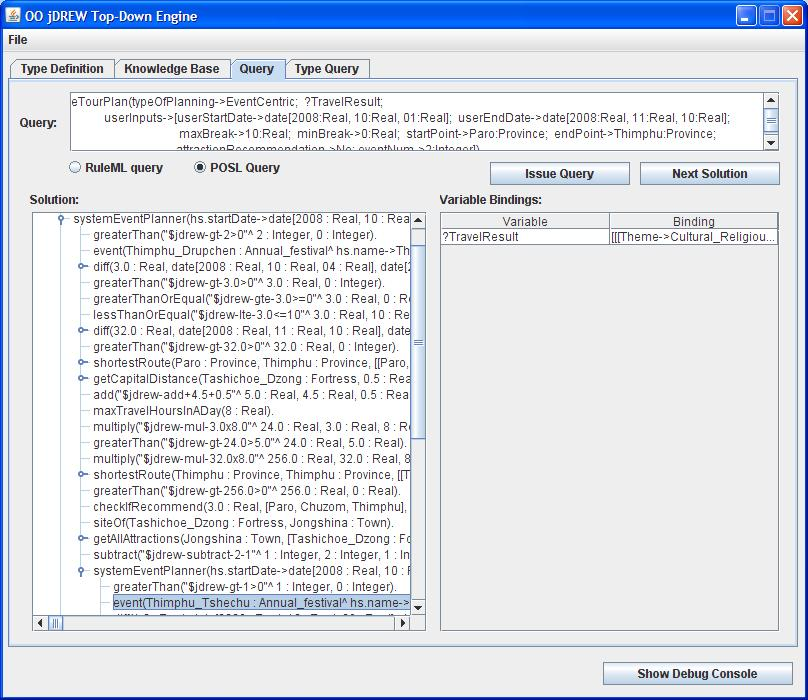
\includegraphics[width=6in]{2EP4}
%\caption {Screenshot for Test Query 2, Next Solution}
%\label{fig:Fig6.3}
%\end{center}
%\end{figure}

%\begin{figure}
%\begin{center}
%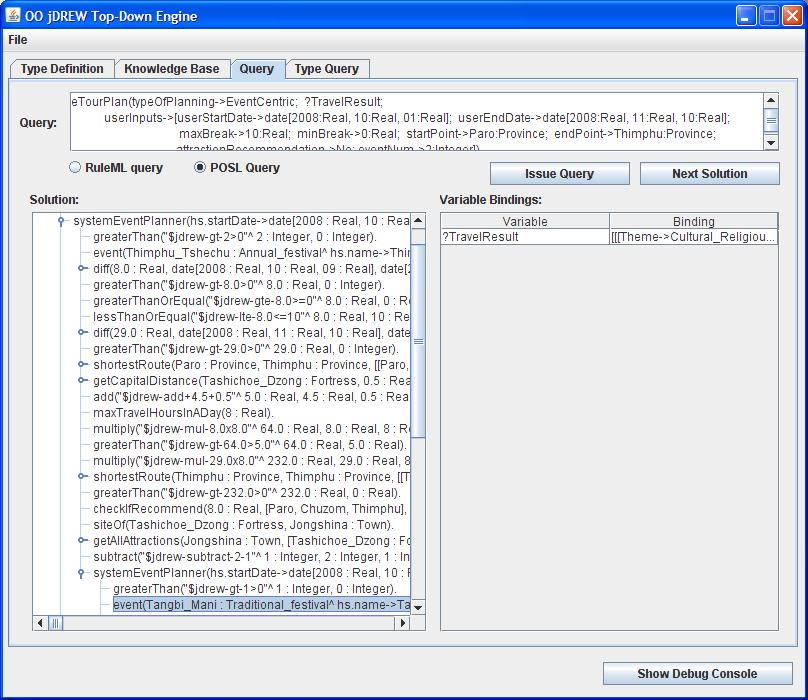
\includegraphics[width=6in]{2EP5}
%\caption {Screenshot for Test Query 2, Next Solution}
%\label{fig:Fig6.3}
%\end{center}
%\end{figure}

%\begin{figure}
%\begin{center}
%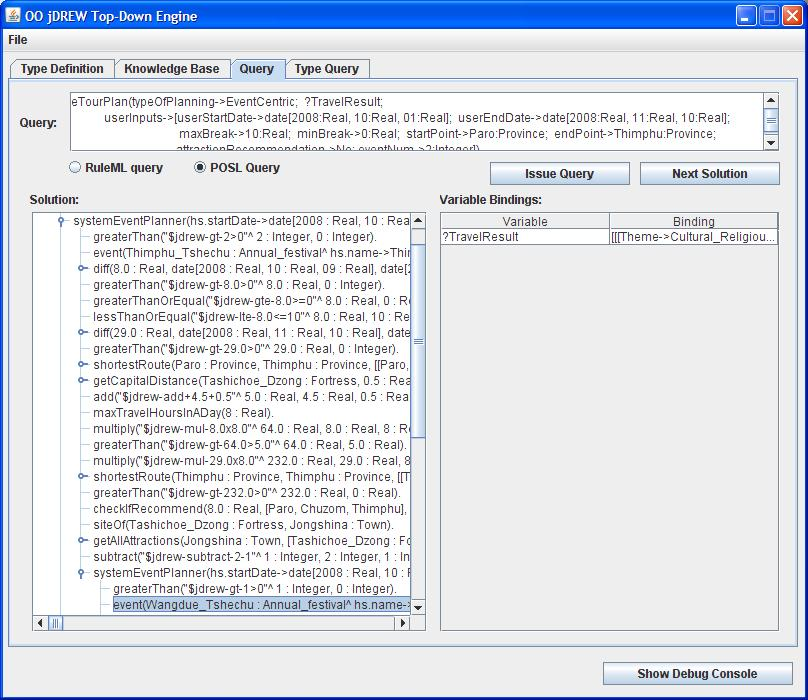
\includegraphics[width=6in]{2EP6}
%\caption {Screenshot for Test Query 2, Next Solution}
%\label{fig:Fig6.3}
%\end{center}
%\end{figure}

\hspace{0.3in}\textbf{Example 3}:\emph{User queries for 3 events within the same dates and constraints as in Example 2,
setting dates from 1st of October to the 10th of November, with a ``maxBreak"' of 10 days and ``minBreak" of 0 days between main events. User selects ``No" for on-route attraction recommendation.}\\

\pagebreak

\hspace{0.3in}\textbf{Test Query 3}:
\begin{small}
\singlespacing
\begin{verbatim}
 eTourPlan(typeOfPlanning->EventCentric; ?TravelResult;
           userInputs->[userStartDate->date[2008:Real, 10:Real, 01:Real];  
                        userEndDate->date[2008:Real, 11:Real, 10:Real]; 
                        maxBreak->10:Real;  
                        minBreak->0:Real; 
                        startPoint->Paro:Province;  
                        endPoin->Thimphu:Province;
                        attractionRecommendation->No; 
                        eventNum->3:Integer]).
\end{verbatim} 
\end{small}

 
\hspace{0.3in}Table 6.17 provides the 5 possible combinations of three events within the user's specified trip dates. Increasing the eventNum to ``four" enforces the system to return a unique solution with four events. The evaluation result for four events is shown in Table 6.18.\\

\hspace{0.3in}\textbf{Test Query 4}:
\begin{small}
\singlespacing
\begin{verbatim}
 eTourPlan(typeOfPlanning->EventCentric; ?TravelResult;
           userInputs->[userStartDate->date[2008:Real, 10:Real, 01:Real];  
                        userEndDate->date[2008:Real, 11:Real, 10:Real]; 
                        maxBreak->10:Real;  
                        minBreak->0:Real; 
                        startPoint->Paro:Province;  
                        endPoin->Thimphu:Province;
                        attractionRecommendation->No; 
                        eventNum->4:Integer]).
\end{verbatim} 
\end{small}

\begin{table} [tbph]
\caption{Evaluation of event-centric travel results}
\centering
\footnotesize
\begin{tabular}{|l|l|l|}
\hline
Event &Event Schedules &Event Sequences\\
 & & $~~~~~$of length\\
 & &$~$ ?EventNum= 4\\
\hline
  1  &Tamshingphala\_Choepa:Traditional\_festival&\\
     &startDate-$>$date[2008:Real,10:Real,08:Real]&\\
   &endDate-$>$date[2008:Real,10:Real,10:Real]&\\
   &province-$>$Bumthang&\\
\hline
  2  &Tangbi\_Mani:Traditional\_festival&\\
     &startDate-$>$date[2008:Real,10:Real,13:Real]&\\
   &endDate-$>$date[2008:Real,10:Real,15:Real]&\\
   &province-$>$Bumthang&\\
\hline
  3  &Thimphu\_Drupchen:Annual\_festival&\textbf{3,4,2,5}\\
     &startDate-$>$date[2008:Real,10:Real,04:Real]&\\
   &endDate-$>$date[2008:Real,10:Real,08:Real]&\\
   &province-$>$Thimphu&\\
\hline
 4  &Thimphu\_Tshechu:Annual\_festival&\\
     &startDate-$>$date[2008:Real,10:Real,09:Real]&\\
   &endDate-$>$date[2008:Real,10:Real,11:Real]&\\
   &province-$>$Thimphu&\\
\hline
 5  &Wangdue\_Tshechu:Annual\_festival&\\
     &startDate-$>$date[2008:Real,10:Real,20:Real]&\\
   &endDate-$>$date[2008:Real, 10:Real, 29:Real]&\\
   &province-$>$WangduePhodrang&\\
\hline
\end{tabular}
\end{table} 
\vspace{-0.5cm}
%\begin{figure}
%\begin{center}
%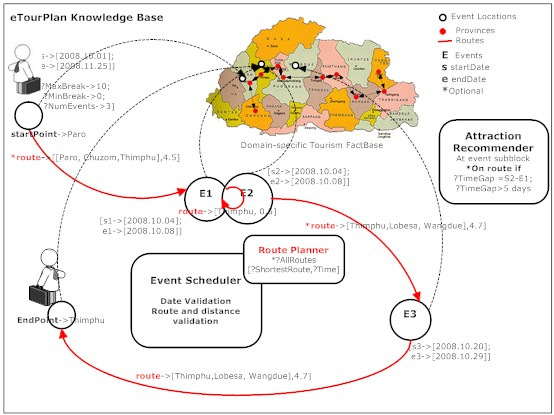
\includegraphics[width=6in]{eTourPlanEventCentric}
%\caption {eTourPlan Event-centric Travel}
%\label{fig:Fig6.3}
%\end{center}
%\end{figure}  

\subsubsection{Execution Times}    

\begin{table} [tbph]
\caption{Execution times for Event-centric Planning}
\centering
\footnotesize
\begin{tabular}{|l|l|}
\hline
  ?NumEvents:Integer & Execution Times (in Milliseconds)\\
\hline
  1& First Solution: 29110\\
   &Next Solution time: 672\\
   &Next Solution time: 719\\
 \hline
  2   & First Solution: 428563 \\
      &Next Solution time: 3563\\
      &Next Solution time: 4797\\
       &Next Solution time: 1282\\
        &Next Solution time: 1359\\
         &Next Solution time: 1250\\
\hline
  3 & First Solution:  4873875\\
     &Next Solution time: 9656\\
     &Next Solution time: 24469\\
     &Next Solution time: 12985\\
\hline
  4 & First Solution:  5428250\\
\hline
\end{tabular} 
\end{table}  

\hspace{0.3in} Although the current version of OO jDREW 0.96 has additional new features (cf. Section 3.3) to support various modes of operations, the reasoning engine performs complete iterative-deepening for each of the predicates, resulting in longer execution times. The OO jDREW team is currently working towards upgrading the current engine to
a system using argument indexing. This will improve the run-time of the eTourPlan rule system. Therefore, complete testing of eTourPlan's functionalities on a faster running OO jDREW is left as future work at this point. 